\graphicspath{{Images/}}

\section{Part 5 - Heuristics in the Adaptive A* }

\textit{Implement and compare Repeated Forward A* and Adaptive A*
with respect to their runtime. Explain your observations in detail, that is, explain what you observed and give a reason for
the observation. Both search algorithms should break ties among cells with the same f-value in favor of cells with larger
g-values and remaining ties in an identical way, for example randomly.}

The source code contains the implementation for Adaptive A*. When the commented section within the main method, responsible for executing both versions across all generated mazes and computing the average time and expanded cells, is uncommented, the ensuing results are as follows.

\begin{figure}[h]
    \centering
    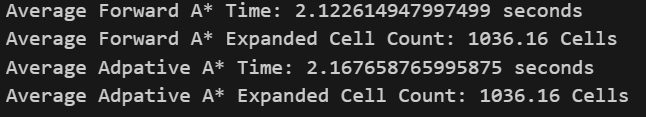
\includegraphics[width=.85\linewidth]{imgs/Results of Forward A vs Adaptive A.png}
    \caption{Comparison of Repeated Forward A* and Adaptive A*}
    \label{fig:my_label}
\end{figure}


In comparing the runtime performance of Repeated Forward A* and Adaptive A*, it is noteworthy that both algorithms exhibited similar outputs. This observation suggests that, within the specific context of the problem space under consideration, the two algorithms demonstrated comparable efficiency in finding optimal paths. The similarity in their runtime performance implies certain characteristics of the environment or the effectiveness of the initial heuristics provided to Adaptive A*.

Repeated Forward A* operates by conducting independent forward A* searches from different start states, ensuring consistency in heuristics throughout each search. While this approach can yield reasonable results, its potential drawback lies in the possibility of re-exploring certain states multiple times, given the independent nature of each search.

On the other hand, Adaptive A* takes a more adaptive approach, initially utilizing consistent heuristics provided by the user. After each search, the algorithm updates action costs if necessary and refines its heuristics based on the knowledge gained. This adaptability allows Adaptive A* to progressively enhance its heuristics over time, leading to a more focused exploration of the state space in subsequent searches. The algorithm's ability to adapt to changes in the environment provides a key advantage over Repeated Forward A*.

Despite the similar runtime outputs, it is essential to consider the potential scenarios where the algorithms may diverge in performance. In cases where the environment remains relatively static and the initial heuristics are well-informed, Repeated Forward A* may deliver competitive results. However, Adaptive A* is anticipated to outperform Repeated Forward A* in dynamic environments or when there is room for improvement in the initial heuristics through experience.

The adaptability of Adaptive A*, evident in its ability to refine heuristics and adapt to changes in action costs over time, positions it as a promising choice for scenarios where the problem space is subject to variations. The consistency in runtime outputs may reflect a stable environment or highly effective initial heuristics, but it is crucial to acknowledge that Adaptive A* holds the potential for superior performance when facing evolving conditions or when continuous refinement of heuristics is beneficial. Both algorithms employ fair tie-breaking strategies, favoring cells with larger g-values and resolving remaining ties randomly.